% !TeX spellcheck = en_GB
\section{Preface}\label{Preface}
In the software world, or more specific, the Java enterprise world, developers tend to abstract access to data in a way that components are interchangeable. A perfect example for such an abstraction is the usage of Object Relational Mappers (ORM). The database specifics are mostly irrelevant to the average developer and the need for native SQL is brought down to a minimum. This makes the switch to a different relational database system (RDBMS) easier in the later stages of a product's life cycle.
\\\\
The Java Persistence API (JPA) went even further by standardising ORMs. First conceived in 2006 \footnote{Wikipedia on Java Persistence API, see~\cite{wiki_jpa}}, it is now the de-facto standard for Object Relational Mappers in Java. The developer doesn't need to know which specific ORM is used in the application, as all the database queries are written against a standardized query API and are therefore portable. This means that not only the database is interchangeable, but even the specific ORM, it is accessed by, is as well.
\\\\
However, this does not mean that all JPA implementations come with the same features. While all of them are JPA compliant (apart from minor bugs), some ship with additional modules to enhance their capabilities. A perfect example for this is the Hibernate Search API aimed at Hibernate ORM users.\footnote{Hibernate ORM project homepage, see~\cite{hibernate_orm}} \footnote{Hibernate Search project homepage, see~\cite{hibernate_search_homepage}}
\\\\
Nowadays, even small applications like online shops need enhanced search capabilities to let the user find more results for a given input.
This is not something a regular RDBMS excels at and Hibernate Search comes into use: It works atop the Hibernate ORM/JPA system and enables the developer to index the domain model for searching. It's not only a mapper from JPA entities to a search index, but also keeps the index up-to-date if something in the database changes.
\\
\begin{figure}[ht]
	\centering
	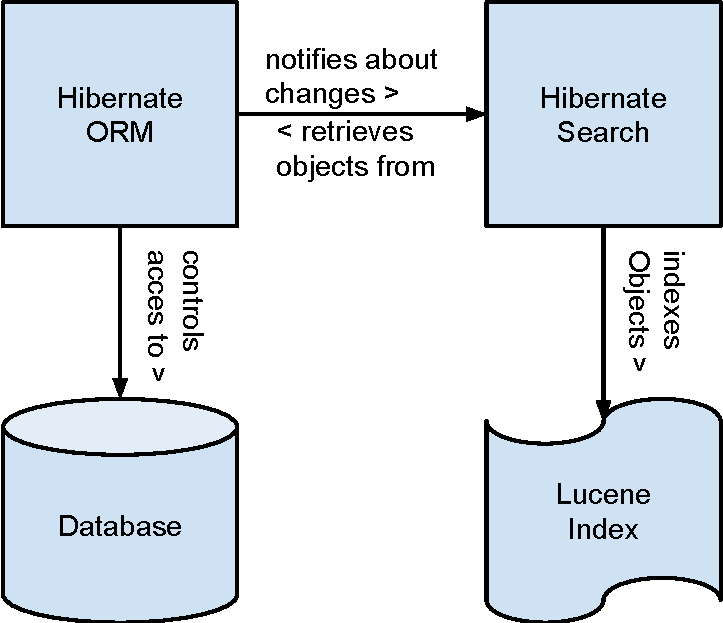
\includegraphics[scale=0.45]{images/hibernate_search_hibernate_schema.pdf}
	\caption{Hibernate Search with Hibernate ORM}
	\label{fig1}
\end{figure}
\pagebreak
\\
Hibernate Search, which is based on the powerful Lucene search toolbox \footnote{sourcecode on Hibernate Search GitHub, see~\cite{hsearch_source_code_git}} \footnote{Hibernate Search FAQ, see~\cite{hibernate_search_faq}}, is a separate project in the Hibernate family and aims to provide a JPA "feeling" in its API as it also incorporates a lot of JPA interfaces in its codebase. However, this does not mean that it is compatible with other JPA providers than Hibernate ORM (apart from Hibernate OGM, the NoSQL JPA mapper of the family).
\\\\
\begin{figure}[ht]
	\centering
	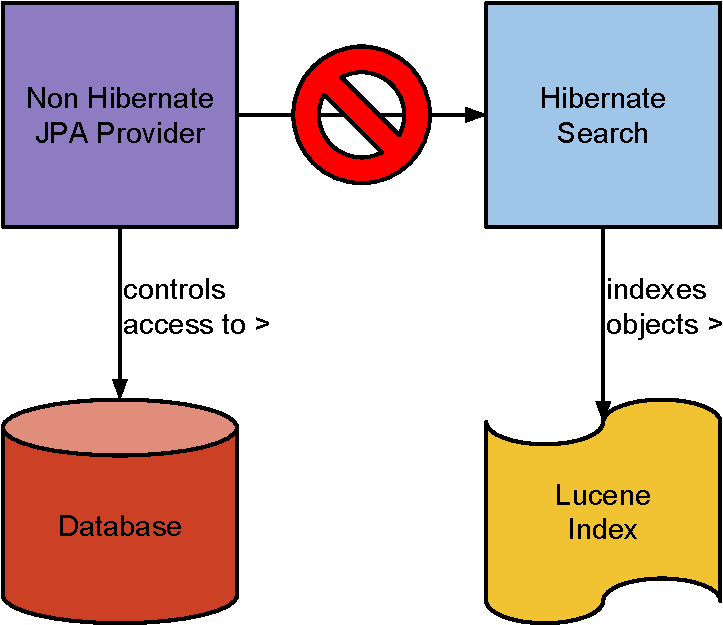
\includegraphics[scale=0.45]{images/hibernate_search_any_jpa_problem_schema.pdf}
	\caption{Hibernate Search's incompatibility with other JPA implementations}
	\label{fig2}
\end{figure}
\\
While using Hibernate Search obviously is beneficial for Hibernate ORM applications, not all developers can bind themselves to a specific JPA implementation in their application. For some, the ability to change implementations might be of strategic importance, for others it could just be sheer preference to use a different JPA implementation.
\\\\
Currently, developers that do not want to bind themselves to Hibernate ORM have to resort to using different full text search systems like native Lucene\footnote{official Lucene website, see~\cite{lucene_apache_org}}, ElasticSearch\footnote{ElasticSearch Java API, see~\cite{elasticsearch_java_api}} or Solr\footnote{Solr Java API, see~\cite{solr_java_api}}. While this is always a viable option, for some applications Hibernate Search would be a much better suit because of its design with a entity structure in mind and the automatic index updating feature, if it just were compatible with generic JPA.
\\\\
When investigating Hibernate Search's project structure
\footnote{Hibernate Search GitHub repository, see~\cite{hsearch_source_code_git}}, we can see that the only module apart from some server-integration modules that depends on any ORM logic is "hibernate-search-orm". The modules that contain the indexing engine, the replication logic, alternative backends, etc. are completely independent from any ORM logic. This means, that most of the codebase could be reused for a generic version of Hibernate Search.

\pagebreak
\noindent
Creating such a generic Hibernate Search is a better approach for a search API on top of JPA rather than rewriting a JPA binding from scratch. Hibernate Search could then act as the standard for fulltext search in the JPA world instead of having a competing API that would just do the same thing in a different style.
\\\\
\begin{figure}[ht]
	\centering
	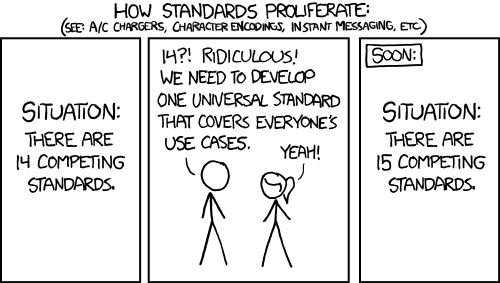
\includegraphics[scale=0.5]{images/competing_standards.png}
	\caption{xkcd.com on competing standards \protect\footnotemark}
	\label{xkcd_standards_fig}
\end{figure}
\footnotetext{xkcd comic \#927, see~\cite{xkcd_competing_standards_source}}
\\
This is why we will show how such a generic version can be built in this thesis. First, we will look at how Hibernate Search's engine can be reused. Then, we will write a standalone version of this engine and finally integrate it with generic JPA.

\fixme{Hier noch ähnlich wie bei einem Paper kurz erklären was in welchem Kapitel passiert}

\pagebreak
~
\pagebreak

\section{Methods} \label{Methods}

\fixme{Überarbeiten, zu unwissenschaftlich}

While developing the generic version of Hibernate Search we are using the following process schema to find the solutions for the all the different problems:

\begin{figure}[ht]
	\centering
	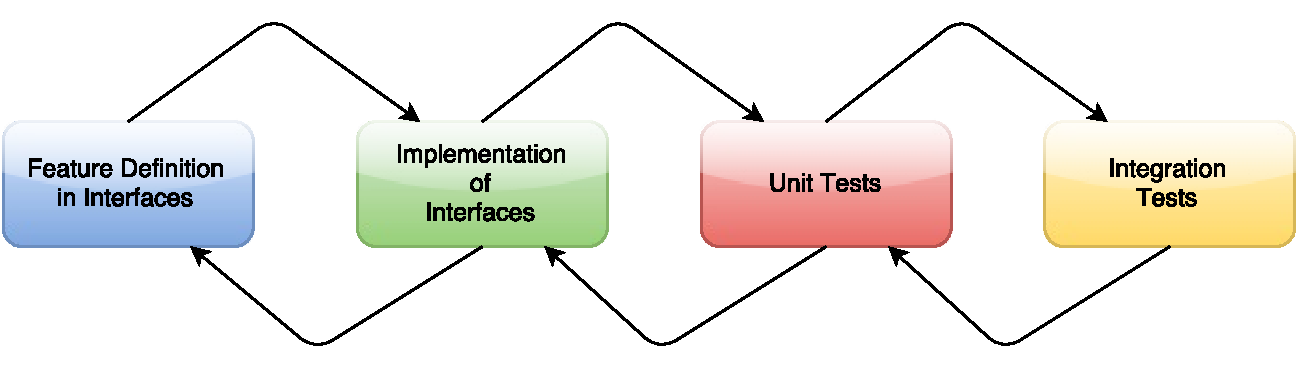
\includegraphics[scale=0.52]{images/work_process.pdf}
	\caption{Development Process of a Feature}
	\label{development_process_of_a_feature}
\end{figure}

\begin{itemize}
	\item \textbf{Analyze Problem}: For every given problem we have to look at all the different aspects of it and try to find the solutions.
	\item \textbf{Define Features in Interfaces}: As building a generic Hibernate Search is a complicated and hard to predict task, creating UML class diagrams would be time consuming as the UML diagrams would be prone to constant changes. In a way, Java interfaces (with the sometimes needed accessory classes and annotations) allow for a rough architectural overview similar to what class diagrams would provide in this case as they allow us to define the ins, outs and side-effects of every method precisely and \textbf{on-the-fly}.
	\\\\
	By defining the features in interfaces first, we achieve complete independence between the implementing classes besides their interfaces and are by default compliant to the \textbf{Open-Closed-Principle} internally: "Modules should be both open (for extension) and closed (for modification)".
	\\\\
	Additionally, while modelling the interfaces we try to be as compliant to the \textbf{Single Responsibility Principle} as possible because it enforces structures that are easy to reuse and change.
	\item \textbf{Implement Interfaces}: Once the interfaces are properly defined, we write implementations for these according to the contracts set.
	\item \textbf{Unit Test}: Each feature has to have a corresponding unit test. These are necessary to test each implementation for the right behaviour (outs and side-effects) for at least one given input.
	\item \textbf{Integration Test}: While Unit-Tests check the behaviour of every \textit{single} feature implementation, integration tests are used to cover the correct behaviour when used together with the other parts of the project in a more real world use case.
\end{itemize}
\noindent
Also note that once a step is finished, that doesn't mean that it is final. As we have seen in the diagram, we can go back and forth between the different steps at will to adapt to specific implementation problems and newly arisen problems that have not been covered before.
\\\\
We choose this kind of on-the-fly approach because it suits the project best: We have to investigate different approaches before we can work out the real solution first. Also because "hibernate-search-engine" is an internal API, we have to be as flexible with our development as possible as some features of it can be different what we might expect in the first place. Our non-strict approach helps us in this aspect as well.

\pagebreak
